\chapter{Statistical
inference for two-way tables}
\label{c_tables}

\section{Introduction}
\label{s_tables_intro}

In this section we continue the discussion of methods of analysis for
two-way contingency tables that was begun in Section
\ref{ss_descr1_2cat_tables}. We will use again the example from the
European Social Survey that was introduced on page
\pageref{p_ess_example}. The two variables in the example are a person's
sex and his or her attitude toward income redistribution measured as an
ordinal variable with five levels. The two-way table of
these variables in the sample is shown again for convenience in Table
\ref{t_sex_attitude_ch4}, including both the frequencies and the conditional
proportions for attitude given sex.

\begin{table}
\caption{Frequencies of respondents in the survey example,
by sex and attitude towards income redistribution. The numbers in
parentheses are conditional proportions
of attitude given sex.}
\label{t_sex_attitude_ch4}
\begin{center}
\begin{tabular}{|l|ccccc|r|}\hline
& \multicolumn{5}{|c|}{\emph{``The government should
take measures}} & \\
& \multicolumn{5}{|c|}{\emph{to reduce differences in income levels''}}
& \\[.3ex]
 & Agree & & Neither agree & & Disagree & \\
Sex & strongly & Agree & nor disagree & Disagree & strongly & Total \\ \hline
Male &  160& 439 & 187 &200  & 41 & 1027 \\
& (0.156) & (0.428) & (0.182) & (0.195) & (0.040) & (1.0) \\
Female & 206 & 651 & 239 & 187 & 34 & 1317\\
& (0.156) & (0.494) & (0.182) & (0.142) & (0.026) & (1.0) \\
\hline
Total & 366 & 1090 & 426 & 387 & 75 & 2344 \\
 & (0.156) & (0.465) & (0.182) & (0.165)& (0.032) & (1.0) \\
\hline
\multicolumn{7}{l}{\scriptsize Data: European Social Survey, Round 5,
2010, UK respondents only.}
\end{tabular}
\end{center}
\vspace*{-3ex}
\end{table}

Unlike in Section \ref{ss_descr1_2cat_tables}, we will now go beyond
description of sample distributions and into
statistical inference. The observed data are thus treated as a sample
from a population, and we wish to draw conclusions about the population
distributions of the variables. In particular, we want to examine
whether the sample provides evidence that the two variables in the table
are associated in the population --- in the example, whether attitude
depends on sex in the population. This is done using a statistical
significance test known as $\chi^{2}$ test of independence.
We will  use it also as a vehicle for introducing
the basic ideas of significance testing in general.

This initial explanation of significance tests is be lengthy and
detailed, because it is important to gain a good understanding of these
fundamental concepts from the beginning. From then on, the same ideas
will be used repeatedly throughout the rest of the course, and in
practically all statistical methods that you may encounter in the
future. You will then be able to draw on what you will have learned in
this chapter, and that learning will also be reinforced through repeated
appearances of the same concepts in different contexts. It will then not
be necessary to restate the basic ideas of the tools of inference in
similar detail. A short summary of the $\chi^{2}$ test considered in
this chapter is given again at the end of the chapter, in Section
\ref{s_tables_summary}.

\section{Significance tests}
\label{s_tables_tests}

A \textbf{significance test} is a method of statistical inference that
is used to assess the plausibility of \emph{hypotheses} about a
population. A hypothesis is a question about
population distributions, formulated as a \emph{claim}
about those distributions. For the test considered in this chapter, the
question is whether or not the two variables in a contingency
table are associated in the population. In the example we want to know
whether men and women have the same
distribution of attitudes towards income redistribution in the
population. For significance testing, this question is expressed as the claim ``The
distribution of attitudes towards income redistribution \emph{is} the
same for men and women'', to which we want to identify the correct
response, either ``Yes, it is'' or ``No, it isn't''.

In trying to answer such questions, we are faced with the
complication that we only have information from a sample. For
example, in Table \ref{t_sex_attitude_ch4} the conditional distributions
of attitude are certainly not identical for men and women. According to
the definition in Section \ref{ss_descr1_2cat_assoc}, this shows that
sex and attitude are associated \emph{in the sample}. This, however,
does not prove that they are also associated \emph{in the population}.
Because of sampling variation, the two conditional distributions are
very unlike to be exactly identical in a sample even if they are the
same in the population. In other words, the hypothesis will not be
exactly true in a sample even if it is true in the population.

On the other hand, some sample values differ from the values claimed by
the hypothesis by so much that it would be difficult to explain them as
a result of sampling variation alone. For example, if we had observed a
sample where 99\% of the men but only 1\% of the women disagreed with
the attitude statement, it would seem obvious that this
should be evidence against the claim that the corresponding probabilities
were nevertheless equal in the population. It would certainly be
stronger evidence against such a claim than the difference of 19.5\%
vs.\ 14.2\% that was actually observed in our sample, which in turn
would be stronger evidence than, say, 19.5\% vs.\ 19.4\%. But
how are we to decide where to draw the line, i.e.\ when to conclude that
a particular sample value is or is not evidence against a hypothesis?
The task of statistical significance testing is to provide explicit and
transparent rules for making such decisions.

\label{p_test_intuition}
A significance test uses a statistic calculated from the sample data (a
\emph{test statistic}) which has the property that its
values will be large if the sample provides evidence against the
hypothesis that is being tested (the \emph{null hypothesis}) and small
otherwise. From a description (a \emph{sampling distribution}) of what
kinds of values the test statistic might have had if the null hypothesis
was actually true in the population, we derive a measure (the
\emph{P-value}) that summarises in one number the strength of evidence
against the null hypothesis that the sample provides. Based on this
summary, we may then use conventional decision rules (\emph{significance
levels}) to make a discrete decision about the null hypothesis about the
population. This decision will be either to \emph{fail to reject} or
\emph{reject} the null hypothesis, in other words to conclude that the observed data are
or are not consistent with the claim about the population stated by the
null hypothesis.

It only remains to put these general ideas into practice by
defining precisely the steps of statistical
significance tests. This is done in the sections below. Since some of
the ideas are somewhat abstract and perhaps initially
counterintuitive, we will introduce them slowly, discussing one at a
time the following basic elements of significance tests:
\begin{itemize}
\item
The hypotheses being tested
\item
Assumptions of a test
\item
Test statistics and their sampling distributions
\item
$P$-values
\item
Drawing and stating conclusions from tests
\end{itemize}
The significance test considered in this chapter is known as the
$\boldsymbol{\chi^{2}}$ \textbf{test of independence} ($\chi^{2}$ is
pronounced ``chi-squared''). It is also known as ``Pearson's
$\chi^{2}$ test'', after Karl Pearson who first proposed it in 1900.\footnote{
\emph{Philosophical Magazine}, Series 5, \textbf{5}, 157--175.
\label{p_pearson} The thoroughly descriptive title of the article is
``On the criterion
that a given system of deviations from the probable in the case of a
correlated system of variables is such that it can be reasonably
supposed to have arisen from random sampling''.
}
We use this test to explain the elements of
significance testing. These principles are, however, not restricted to
this case, but are entirely general. This means that all of the
significance tests you will learn on this course or elsewhere have the
same basic structure, and differ only in their details.


\section{The $\chi^{2}$ test of independence}
\label{s_tables_chi2test}

\subsection{Hypotheses}
\label{ss_tables_chi2test_null}

\subsubsection{The null hypothesis and the alternative hypothesis}

The technical term for the hypothesis that is tested in statistical
significance testing is the \textbf{null hypothesis}. It is often
denoted $H_{0}$. The null hypothesis is a specific claim about
population distributions. The $\chi^{2}$ test of independence concerns
the association between two categorical variables, and its null
hypothesis is that there is no such association in the population.

In
the context of this test, it is conventional to use alternative
terminology where the variables are said to be \textbf{statistically
independent} when there is no association between them, and
\textbf{statistically dependent} when they are associated. Often the
word ``statistically'' is omitted, and we talk simply of
variables being independent or dependent. In this language, the null
hypothesis of the $\chi^{2}$ test of independence is that
\begin{equation}
H_{0}: \;\text{The variables are statistically independent in the
population}.
\label{H0_chi2}
\end{equation}
In our example the null hypothesis is thus that a person's sex and his
or her attitude toward income redistribution are independent in the
population of adults in the UK.

The null hypothesis (\ref{H0_chi2}) and the $\chi^{2}$ test itself are
symmetric in that there is no need to designate one of the
variables as explanatory and the other as the response variable. The
hypothesis can, however, also be expressed in a form which does make use
of this distinction. This links it more clearly with the definition of
associations in terms of conditional
distributions. In this form, the null
hypothesis (\ref{H0_chi2}) can also be stated as the claim that the
conditional distributions of the response variable are the same at
all levels of the explanatory variable, i.e.\ in our example as
\[
H_{0}: \;\text{The conditional distribution of attitude is the same for
men as for women}.
\]
The hypothesis could also be expressed for the conditional distributions
the other way round, i.e.\ here that the distribution of sex is the same
at all levels of the attitude. All three versions of the null hypothesis
mean the same thing for the purposes of the significance test.
Describing the hypothesis in particular terms is useful purely for easy
interpretation of the test and its conclusions in specific examples.

As well as the null hypothesis, a significance test usually involves
an \textbf{alternative hypothesis}, often denoted $H_{a}$. This
is in some sense the opposite of the null hypothesis, which
indicates the kinds of observations that will be taken as evidence against
$H_{0}$. For the $\chi^{2}$ test of independence this is simply the logical
opposite of (\ref{H0_chi2}), i.e.\
\begin{equation}
H_{a}: \;\text{The variables are not statistically independent in the
population}.
\label{Ha_chi2}
\end{equation}
In terms of conditional distributions, $H_{a}$ is that the conditional
distributions of one variable given the other are not all identical,
i.e.\ that for at least one pair of levels of the explanatory variable
the conditional probabilities of at least one category of the response
variable are not the same.

\subsubsection{Statistical hypotheses and research hypotheses}

The word ``hypothesis'' appears also in research design and
philosophy of science. There a \textbf{research hypothesis} means a
specific claim or prediction about observable quantities, derived
from subject-matter theory. The prediction is then compared to
empirical observations. If the two are in reasonable agreement, the
hypothesis and corresponding theory gain support or
\emph{corroboration}; if observations disagree with the predictions,
the hypothesis is \emph{falsified} and the theory must eventually be
modified or abandoned. This role of research hypotheses is, especially
in the philosophy of science originally associated with Karl Popper, at
the heart of the scientific method. A theory which does not
produce empirically falsifiable hypotheses, or fails to be
modified even if its hypotheses are convincingly falsified, cannot be
considered scientific.

Research hypotheses of this kind are closely related to the kinds of
\textbf{statistical hypotheses} discussed above. When
empirical data are quantitative, decisions about research hypotheses are
in practice usually made, at least in part, as decisions about
statistical hypotheses implemented through sinificance tests. The
falsification and corroboration of research hypotheses are then
parallelled by rejection and non-rejection of statistical hypotheses.
The connection is not, however, entirely straightforward, as
there are several differences between research hypotheses and
statistical hypotheses:
\begin{itemize}
\item
Statistical significance tests are also often used for testing
hypotheses which do not correspond to any theoretical research
hypotheses. Sometimes the purpose of the test is just to identify those
observed differences and regularities which are large enough to deserve
further discussion. Sometimes claims stated as null hypotheses are
interesting for reasons which have nothing to do with theoretical
predictions but rather with, say, normative or policy goals.
\item
Research hypotheses are typically stated as predictions about
theoretical concepts. Translating them into testable statistical
hypotheses requires further operationalisation of these concepts. First,
we need to decide how the concepts are to be measured. Second, any test
involves also assumptions which are imposed not
by substantive theory but by constraints of
statistical methodology. Their appropriateness for the data at hand
needs to be assessed separately.
\item
The conceptual connection is clearest when the research hypothesis
matches
the null hypothesis of a test in general form. Then the research hypothesis
remains unfalsified as long as the null
hypothesis remains not rejected, and gets
falsified when the null hypothesis is rejected. Very often, however, the
statistical hypotheses are for technical reasons
defined the other way round. In particular,
for significance tests that are about
associations between variables, a research hypothesis is typically
that there \emph{is} an association between particular variables,
whereas the null hypothesis is that there is \emph{no} association
(i.e.\ ``null'' association). This
leads to the rather confusing situation where the research hypothesis is
supported when the null hypothesis is rejected, and possibly falsified when the
null hypothesis is not rejected.
\end{itemize}


\subsection{Assumptions of a significance test}
\label{ss_tables_chi2test_ass}

In the following discussion we will sometimes refer to Figure
\ref{f_spsschi2}, which shows SPSS output for the $\chi^{2}$ test of
independence for the data in Table \ref{t_sex_attitude_ch4}. Output for
the test is shown on the line labelled ``Pearson Chi-Square'', and ``N
of valid cases'' gives the sample size $n$. The other entries in the
table are output for other tests that are not discussed here, so they
can be ignored.

\begin{figure}
\caption{SPSS output of the $\chi^{2}$ test of independence (here labelled
``Pearson Chi-square'') for the data in Table \ref{t_sex_attitude_ch4}.}
\label{f_spsschi2}
\begin{center}
%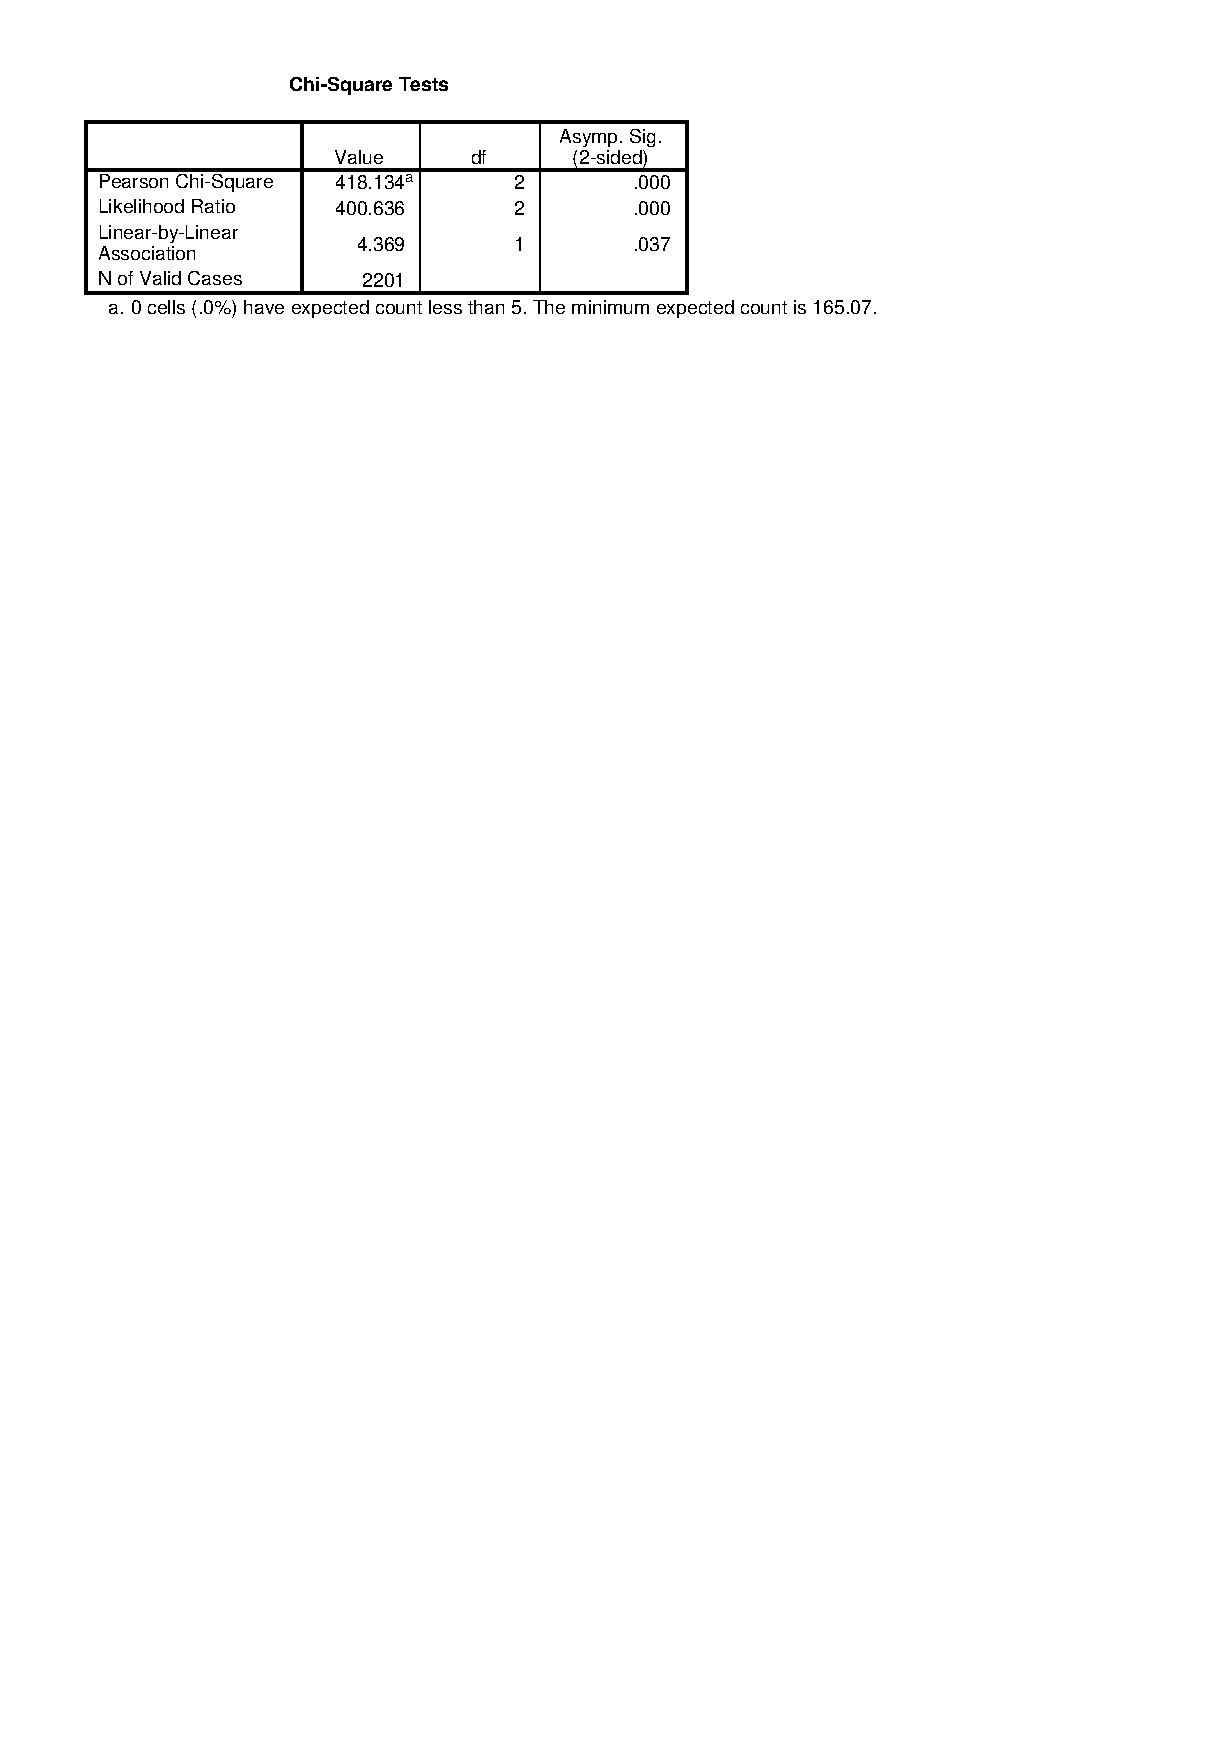
\includegraphics[bb=10 11 585 831, width=130mm]{spsschi2.eps}
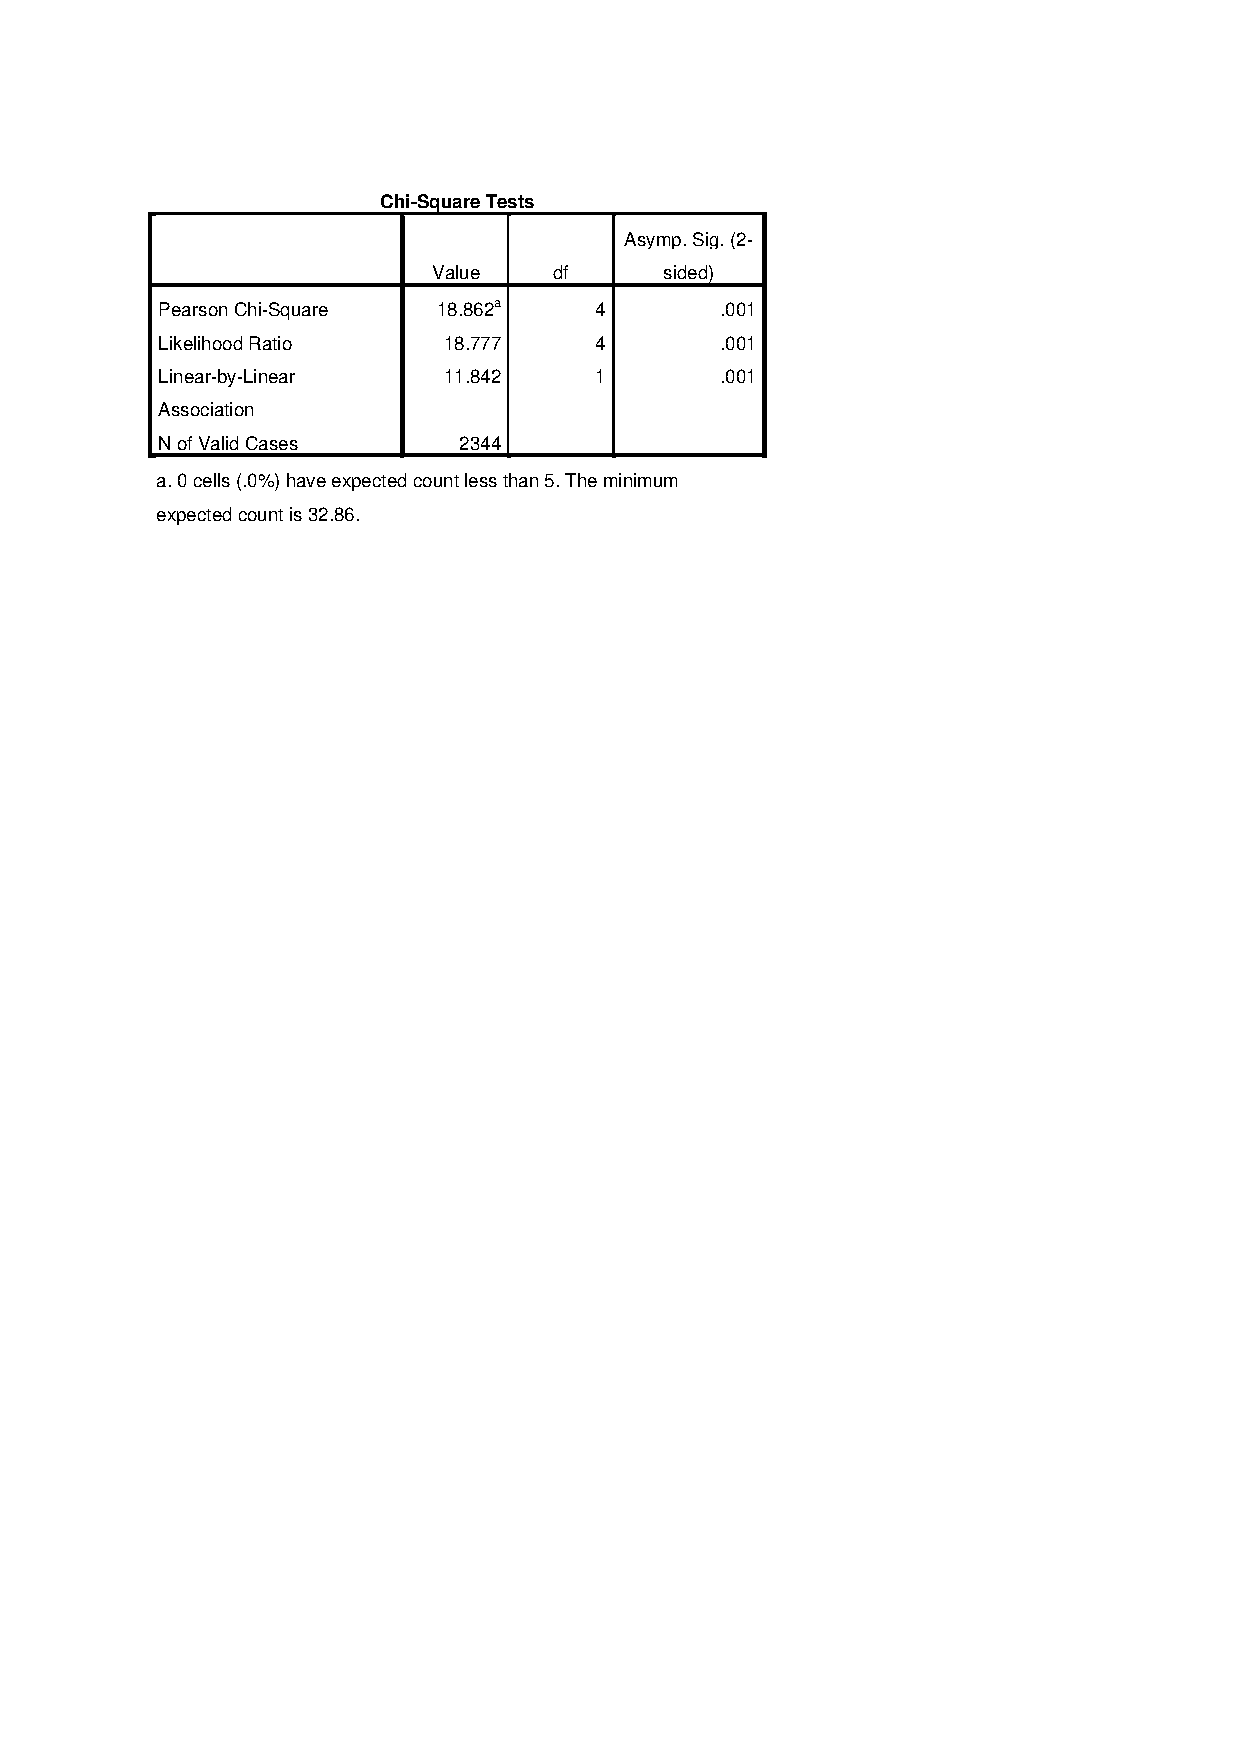
\includegraphics[width=100mm]{chi2test_ess}
\vspace*{-2ex}
\end{center}
\end{figure}


When we apply any significance test, we need to be aware of its
\textbf{assumptions}. These are conditions on the data which are not
themselves being tested, but which need to be approximately satisfied
for the conclusions from the test to be valid. Two broad types of such
assumptions are particularly common. The first kind are assumptions
about the measurement levels and population distributions of the
variables. For the $\chi^{2}$ test of independence these are relatively
mild. The two variables must be categorical variables. They can have any
measurement level, although in most cases this will be either nominal or
ordinal. The test makes no use of the ordering of the categories, so it
effectively treats all variables as if they were nominal.

\label{p_chi2_fesize}
The second common class of assumptions are conditions on the sample size. Many significance tests are appropriate
only if this is sufficiently large. For the $\chi^{2}$ test,
the expected frequencies $f_{e}$ (which will be defined below) need
to be large enough in \emph{every cell} of the table. A common rule of
thumb is that the test can be safely used if all expected frequencies
are at least 5. Another, slightly more lenient rule requires only that
no more than 20\% of the expected frequencies are less than 5, and that
none are less than 1. These conditions can easily be checked with the
help of SPSS output for the $\chi^{2}$ test, as shown in Figure
\ref{f_spsschi2}. This gives information on the number and proportion of
expected frequencies (referred to as ``expected counts'') less than
five, and also the size of the smallest of them. In our example the
smallest expected frequency is about 33, so
the sample size condition is easily satisfied.

When the expected frequencies do not satisfy these conditions, the
$\chi^{2}$ test is not fully valid, and the results should be treated
with caution (the reasons for this will be discussed below). There are
alternative tests which do not rely on these large-sample assumptions,
but they are beyond the scope of this course.

In general, the hypotheses of a test define the questions it can answer,
and its assumptions indicate the types of data it is appropriate for.
Different tests have different hypotheses and assumptions, which need to
be considered in deciding which test is appropriate for a given
analysis. We will introduce a number of different significance tests in
this coursepack, and give guidelines for choosing between them.

\subsection{The test statistic}
\label{ss_tables_chi2test_stat}


A \textbf{test statistic} is a number calculated from the sample (i.e.\
a statistic in the sense defined on page \pageref{p_statistic}) which is
used to test a null hypothesis. We we will describe the calculation of
the $\chi^{2}$ test statistic step by step, using the data in Table
\ref{t_sex_attitude_ch4} for illustration.
All of the elements of the test statistic for this example
are shown in Table \ref{t_sex_attitude_chi2}. These elements are
\begin{itemize}
\item
The \textbf{observed frequencies}, denoted $f_{o}$,
one for each cell of the table. These are simply the observed
cell counts (compare the $f_{o}$ column of Table \ref{t_sex_attitude_chi2} to
the counts in Table \ref{t_sex_attitude_ch4}).
\item
The \textbf{expected frequencies} $f_{e}$, also one for each cell. These
are cell counts in a hypothetical table which would show no association between
the variables. In other words, they represent a table for a sample which
would exactly agree with the null hypothesis of independence in the
population. To explain how the expected frequencies are calculated,
consider the cell in Table \ref{t_sex_attitude_ch4} for Male respondents
who strongly agree with the statement. As discussed above, if the null
hypothesis of independence is true in the population, then the
conditional probability of strongly agreeing is the same for both men
and women. This also implies that it must then be equal to
the overall (marginal) probability of strongly agreeing.
The sample version of this is that the proportion who strongly
agree should be
the same for men as among all respondents overall. This overall
proportion in Table \ref{t_sex_attitude_ch4} is $366/2344=0.156$. If this
proportion applied also to the 1027 male respondents, the number of
of them who strongly agreed would be
\[
f_{e} = \left(\frac{366}{2344}\right)\times 1027 =
\frac{366\times 1027}{2344}=160.4.
\]
Here 2344 is the total sample size, and 366 and 1027 are the marginal
frequencies of strongly agreers and male respondents respectively, i.e.\
the two marginal totals corresponding to the cell (Male, Strongly
agree). The same rule applies also in general: the expected frequency
for any cell in this or any other table is calculated as the product of
the row and column totals corresponding to the cell, divided by the
total sample size.
\item
The difference $f_{o}-f_{e}$ between observed and expected frequencies
for each cell. Since $f_{e}$ are the cell counts in a table which exactly
agrees with the null hypothesis, the differences indicate how closely
the counts $f_{o}$ actually observed agree with $H_{0}$. If the
differences are small, the observed data are consistent with the null
hypothesis, whereas large differences indicate evidence against it.
The test statistic will be obtained by aggregating information about these
differences across all the cells of the table. This cannot, however, be
done by adding up the differences themselves, because positive
($f_{o}$ is larger than $f_{e}$)
and negative
($f_{o}$ is smaller than $f_{e}$) differences
will always exactly cancel each other
out (c.f.\ their sum on the last row of Table \ref{t_sex_attitude_chi2}). Instead, we
consider...
\item
...the squared differences $(f_{o}-f_{e})^{2}$. This
removes the signs from the differences, so that the squares of
positive and negative differences which are equally far from zero will
be treated as equally strong evidence against the null hypothesis.
\item
Dividing the squared differences by the expected frequencies, i.e.\
$(f_{o}-f_{e})^{2}/f_{e}$. This is an essential but not particularly
interesting scaling exercise, which expresses the sizes of the squared
differences relative to the sizes of $f_{e}$ themselves.
\item
Finally, aggregating these quantities
to get the $\chi^{2}$ test statistic
\begin{equation}
\chi^{2} = \sum \frac{(f_{o}-f_{e})^{2}}{f_{e}}.
\label{chi2}
\end{equation}
Here the summation sign $\Sigma$ indicates that $\chi^{2}$ is obtained
by adding up the quantities $(f_{o}-f_{e})^{2}/f_{e}$ across all the cells of
the table.
\end{itemize}

\begin{table}
\caption{Calculating the $\chi^{2}$ test statistic for Table
\ref{t_sex_attitude_ch4}. In the second column,
SA, A, 0, D, and SD are abbreviations
for Strongly agree, Agree, Neither agree nor disagree, Disagree and
Strongly disagree respectively.}
\label{t_sex_attitude_chi2}
\begin{center}
\begin{tabular}{|lc|rrrrr|}\hline
\multicolumn{2}{|c|}{Cell} & & & & & \\
Sex & Attitude & $f_{o}$ & $f_{e}$ & $f_{o}-f_{e}$ & $(f_{o}-f_{e})^{2}$ &
$(f_{o}-f_{e})^{2}/f_{e}$\\
\hline
Male & SA & 160 & 160.4 & $-0.4$& 0.16& 0.001 \\
Male & A & 439 & 477.6 & $-38.6$ & 1489.96& 3.120 \\
Male & 0 & 187 & 186.6 & 0.4& 0.16& 0.001 \\
Male & D & 200 & 169.6 & 30.4& 924.16& 5.449 \\
Male & SD & 41 & 32.9 & 8.1& 65.61& 1.994 \\[.5ex]
Female & SA & 206 & 205.6 & 0.4& 0.16 & 0.001 \\
Female & A & 651 & 612.4 & 38.6& 1489.96& 2.433 \\
Female & 0 & 239 & 239.4 & $-0.4$& 0.16& 0.001 \\
Female & D & 187 & 217.4 & $-30.4$& 924.16& 4.251 \\
Female & SD & 34 & 42.1 & $-8.1$& 65.61& 1.558 \\
\hline
& Sum & 2344& 2344 & 0 & 4960.1& $\chi^{2}=18.81$ \\
\hline
\end{tabular}
\end{center}
\end{table}

The calculations can be done even by hand, but we will
usually leave them to a computer. The last column of Table
\ref{t_sex_attitude_chi2} shows that for Table \ref{t_sex_attitude_ch4}
the test statistic is $\chi^{2}=18.81$ (which includes some rounding
error, the correct value is 18.862). In the SPSS output in Figure
\ref{f_spsschi2}, it is given in the ``Value'' column of the
``Pearson Chi-Square'' row.


\subsection{The sampling distribution of the test statistic}
\label{ss_tables_chi2test_sdist}

We now know that the value of the $\chi^{2}$ test statistic in the
example is 18.86. But what does that mean? Why is the test statistic
defined as (\ref{chi2}) and not in some other form? And what does the
number mean? Is 18.86 small or large, weak or strong evidence against
the null hypothesis that sex and attitude are independent in the
population?

In general, a test
statistic for any null hypothesis should satisfy two
requirements:\label{p_2reqs}
\begin{enumerate}
\item
The value of the test statistic should be small when evidence against
the null hypothesis is weak, and large when this evidence is strong.
\item
The sampling distribution of the test statistic should be known and of
convenient form when the null hypothesis is true.
\end{enumerate}
Taking the first requirement first, consider the form of (\ref{chi2}).
The important part of this are the squared differences
$(f_{o}-f_{e})^{2}$ for each cell of the table. Here the expected
frequencies $f_{e}$ reveal what the table would look like if the
sample was in perfect agreement with the claim of independence in the
population, while the observed frequencies $f_{o}$ show what the
observed table actually does look like. If $f_{o}$ in a cell is close to
$f_{e}$, the squared difference is small and the cell contributes only a
small addition to the test statistic. If $f_{o}$ is
very different from $f_{e}$ --- either much smaller or much larger than
it --- the squared difference and hence the cell's contribution to the
test statistic are large.

Summing the contributions over all the cells, this implies that the
overall value of the test statistic is small when the observed
frequencies are close to the expected frequencies under the null
hypothesis, and large when at least some of the observed frequencies are
far from the expected ones. (Note also that the smallest possible value
of the statistic is 0, obtained when the observed and the expected
frequency are exactly equal in each cell.) It is thus \emph{large}
values of $\chi^{2}$ which should be regarded as evidence \emph{against}
the null hypothesis, just as required by condition 1 above.

Turning then to condition 2, we first need to explain what is meant by
``sampling distribution of the test statistic ... when the null
hypothesis is true''. This is really the conceptual crux of significance
testing. Because it is both so important and relatively abstract, we
will introduce the concept of a sampling distribution in some detail,
starting with a general definition and then focusing on the case of test
statistics in general and the $\chi^{2}$ test in particular.

\subsubsection{Sampling distribution of statistic: General definition}

The $\chi^{2}$ test statistic (\ref{chi2}) is a \emph{statistic} as
defined defined on page \pageref{p_statistic}, that is a number
calculated from data in a sample. Once we have observed a sample, the
value of a statistic in that sample is known, such as the 18.862 for
$\chi^{2}$ in our example.

However, we also realise that this value would have been different if the
sample had been different, and also that the sample could indeed have
been different because the sampling is a process that involves
randomness. For example, in the actually observed sample in Table
\ref{t_sex_attitude_ch4} we had 200 men who disagreed with the statement
and 41 who strongly disagreed with it. It is easily imaginable that
another random sample of 2344 respondents from the same population could
have given us frequencies of, say, 195 and 46 for these cells instead.
If that had happened, the value of the $\chi^{2}$ statistic would have
been 19.75 instead of 18.86. Furthermore, it also seems intuitively
plausible that not all such alternative values are equally likely for
samples from a given population. For example, it seems quite improbable
that the population from which the sample in Table
\ref{t_sex_attitude_ch4} was drawn would instead produce a sample which
also had 1027 men and 1317 women but where all the men strongly
disagreed with the statement (which would yield $\chi^{2}=2210.3$).

The ideas that different possible samples would give different values of
a sample statistic, and that some such values are more likely than
others, are formalised in the concept of a sampling distribution:
\begin{itemize}
\item
The \textbf{sampling distribution of a statistic} is the distribution of
the statistic (i.e.\ its possible values and the proportions with which
they occur) in the set of all possible random samples of the same size
from the population.
\end{itemize}
To observe a sampling distribution of a statistic, we would thus need to
draw samples from the population over and over again, and calculate
the value of the statistic for each such sample, until we had a good
idea of the proportions with which different values of the statistic
appeared in the samples. This is clearly an entirely hypothetical
exercise in most real examples where we have just one sample of actual
data, whereas the number of possible samples of that size is essentially
or actually infinite. Despite this, statisticians can find out
what sampling distributions would look like,
under specific assumptions about the population. One way to do so is
through mathematical derivations. Another is a \emph{computer simulation}
where we use a computer program to draw a large number of samples from
an artificial population, calculate the value of a statistic
for each of them, and examine the distribution of the statistic across these
repeated samples. We will make use of both of these approaches below.

\subsubsection{Sampling distribution of a test statistic under the null
hypothesis}

The sampling distribution of any statistic depends primarily on what the
population is like. For test statistics, note that requirement 2 above
mentioned only the situation where the null hypothesis is true. This is
in fact the central conceptual ingredient of significance testing. The
basic logic of drawing conclusions from such tests is that we consider
what we would expect to see if the null hypothesis was in fact true in
the population, and compare that to what was actually observed in our
sample. The null hypothesis should then be rejected if the observed data
would be surprising (i.e.\ unlikely) if the null hypothesis was actually
true, and not rejected if the observed data would not be surprising
under the null hypothesis.

We have already seen that the $\chi^{2}$ test statistic is in effect
a measure of the discrepancy between what is expected under the null
hypothesis and what is observed in the sample. All test statistics for
any hypotheses have this property in one way or another. What then
remains to be determined is exactly how surprising or otherwise the observed data
are relative to the null hypothesis. A measure of this is derived from the
sampling distribution of the test statistic \emph{under the null
hypothesis}. It is the only sampling distribution that is needed for
carrying out a significance test.

\subsubsection{Sampling distribution of the $\chi^{2}$ test statistic under independence}

For the $\chi^{2}$ test, we need the sampling distribution of the test
statistic (\ref{chi2}) under the independence null hypothesis
(\ref{H0_chi2}). To make these ideas a little more concrete, the upper
part of Table \ref{t_sex_attitude_H0pop} shows the crosstabulation of
sex and attitude in our example for a finite population where the null
hypothesis holds. We can see that it does because the two
conditional distributions for attitude, among men and among women, are
the same (this is the only aspect of the distributions that matters for this
demonstration; the exact values of the probabilities are otherwise
irrelevant). These are of course hypothetical population distributions,
as we do not know the true ones. We also do not claim that this
hypothetical population is even close to the true one. The whole point
of this step of hypothesis testing is to set up a population where the
null hypothesis holds as a fixed point of comparison, to see what
samples from such a population would look like and how they compare with
the real sample that we have actually observed.

\begin{table}[t]
\caption{Attitude towards income redistribution by sex (with row
proportions in parentheses), in a hypothetical
population of 50 million people where sex and attitude are independent,
and in one random sample from this population.}
\label{t_sex_attitude_H0pop}

\vspace*{1ex}
\emph{Population (frequencies are in millions of people):}
\begin{center}
\begin{tabular}{|l|ccccc|r|}\hline
& \multicolumn{5}{|c|}{\emph{``The government should
take measures}} & \\
& \multicolumn{5}{|c|}{\emph{to reduce differences in income levels''}}
& \\[.3ex]
 & Agree & & Neither agree & & Disagree & \\
Sex & strongly & Agree & nor disagree & Disagree & strongly & Total \\ \hline
Male & 3.744& 11.160& 4.368& 3.960& 0.768&  24.00\\
 & (0.156) & (0.465) & (0.182) & (0.165)& (0.032) & (1.0)  \\[.5ex]
Female & 4.056& 12.090& 4.732& 4.290& 0.832& 26.00\\
 & (0.156) & (0.465) & (0.182) & (0.165)& (0.032) & (1.0) \\
\hline
Total & 7.800 & 23.250 &  9.100&  8.250& 1.600 & 50 \\
 & (0.156) & (0.465) & (0.182) & (0.165)& (0.032) & (1.0) \\
\hline
\end{tabular}
\end{center}
\vspace*{1ex}
\emph{Sample:}
\begin{center}
\begin{tabular}{|l|ccccc|r|}\hline
 & Agree & & Neither agree & & Disagree & \\
Sex & strongly & Agree & nor disagree & Disagree & strongly & Total \\ \hline
Male & 181& 505& 191& 203& 41& 1121 \\
 & (0.161) & (0.450) & (0.170) & (0.181)& (0.037) & (1.0)  \\[.5ex]
Female & 183& 569& 229& 202& 40& 1223\\
 & (0.150) & (0.465) & (0.187) & (0.165)& (0.033) & (1.0) \\
\hline
Total & 364& 1074& 420& 405& 81& 2344 \\
 & (0.155) & (0.458) & (0.179) & (0.173)& (0.035) & (1.0) \\
\hline
\multicolumn{7}{l}{\small $\chi^{2}=2.8445$}
\end{tabular}
\end{center}
\vspace*{-3ex}
\end{table}

In the example we have a sample of 2344 observations, so to match that
we want to identify the sampling distribution of the $\chi^{2}$
statistic in random samples of size 2344 from the population like the
one in the upper part of Table \ref{t_sex_attitude_H0pop}. The lower
part of that table shows one such sample. Even though it comes from a
population where the two variables are independent, the same is not
exactly true in the sample: we can see that the conditional sample
distributions are not the same for men and women. The value of the
$\chi^{2}$ test statistic for this simulated sample is 2.8445.

Before we proceed with the discussion of the sampling distribution of
the $\chi^{2}$ statistic, we should note that it will be a
\emph{continuous} probability distribution. In other words, the number
of distinct values that the test statistic can have in different samples
is so large that their distribution is clearly effectively continuous.
This is true even though the two \emph{variables} in the contingency
table are themselves categorical. The two distributions, the population
distribution of the variables and the sampling distribution of a test
statistic, are quite separate entities and need not resemble each other.
We will consider the nature of continuous probability distributions in
more detail in Chapter \ref{c_means}. In this chapter we will discuss
them relatively superficially and only to the extent that is absolutely
necessary.

Figure \ref{f_chisampld} shows what we observe if do a computer
simulation to draw many more samples from the population in Table
\ref{t_sex_attitude_H0pop}. The figure shows the histogram of the values
of the $\chi^{2}$ test statistic calculated from 100,000 such samples.
We can see, for example,  that $\chi^{2}$ is between 0 and 10 for most of the samples,
and larger than that for only a small proportion of them. In
particular, we note already that the value $\chi^{2}=18.8$ that was
actually observed in the real sample occurs very rarely if samples are
drawn from a population where the null hypothesis of independence holds.


\begin{figure}[t]
\caption{Example of the sampling distribution of the $\chi^{2}$ test
statistic for independence. The
plot shows a histogram of the values of the statistic in 100,000
simulated samples
of size $n=2344$ drawn from the population distribution in the upper
part of Table \ref{t_sex_attitude_H0pop}.
Superimposed on the histogram
is the curve of the approximate sampling
distribution, which is  the $\chi^{2}$ distribution with 4 degrees of
freedom.
}
\label{f_chisampld}
\begin{center}
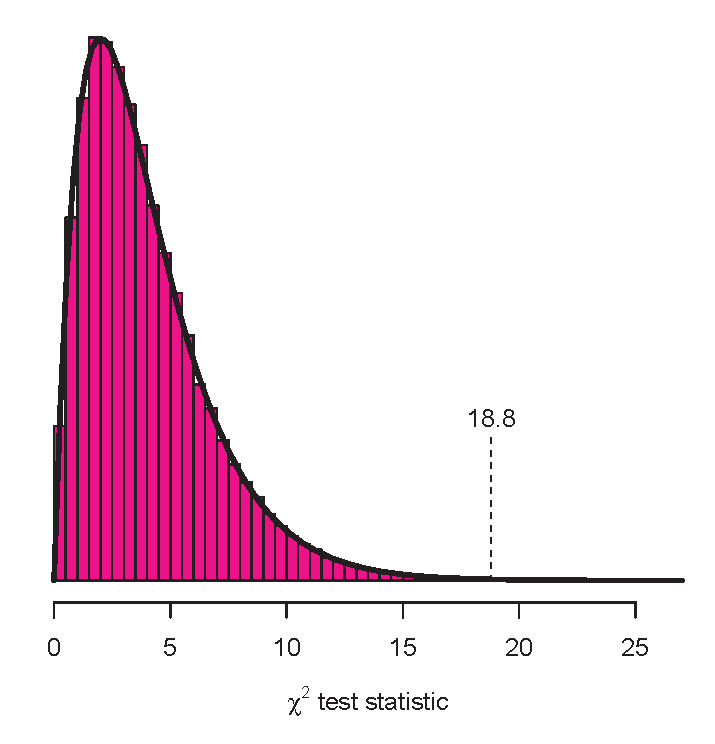
\includegraphics[width=8.5cm]{chi2sims}
\end{center}
\vspace*{-3ex}
\end{figure}

The form of the sampling distribution can also be derived
through mathematical arguments. These show that
for any two-way contingency table, the approximate sampling distribution
of the $\chi^{2}$ statistic is a member of a class of continuous
probability distributions known as the $\boldsymbol{\chi}^{2}$
\textbf{distributions} (the same symbol $\chi^{2}$ is rather
confusingly used to refer both to the test statistic and its sampling
distribution). The $\chi^{2}$ distributions are a family of individual
distributions, each of which is identified by a number known as the
\textbf{degrees of freedom} of the distribution.
Figure \ref{f_chi2dists} shows the probability curves of some $\chi^{2}$
distributions (what such curves mean is explained in more detail below,
and in Chapter \ref{c_means}). All of the distributions are skewed to the right, and the
shape of a particular curve depends on its degrees of feedom. All of the
curves give non-zero probabilites only for positive values of the
variable on the horizontal axis, indicating that the value of a
$\chi^{2}$-distributed variable can never be negative. This is
appropriate for the $\chi^{2}$ test statistic (\ref{chi2}), which is
also always non-negative.

\begin{figure}
\caption{Probability curves of some $\chi^{2}$ distributions with
different degrees of freedom (df).}
\label{f_chi2dists}
\vspace*{-2ex}
\begin{center}
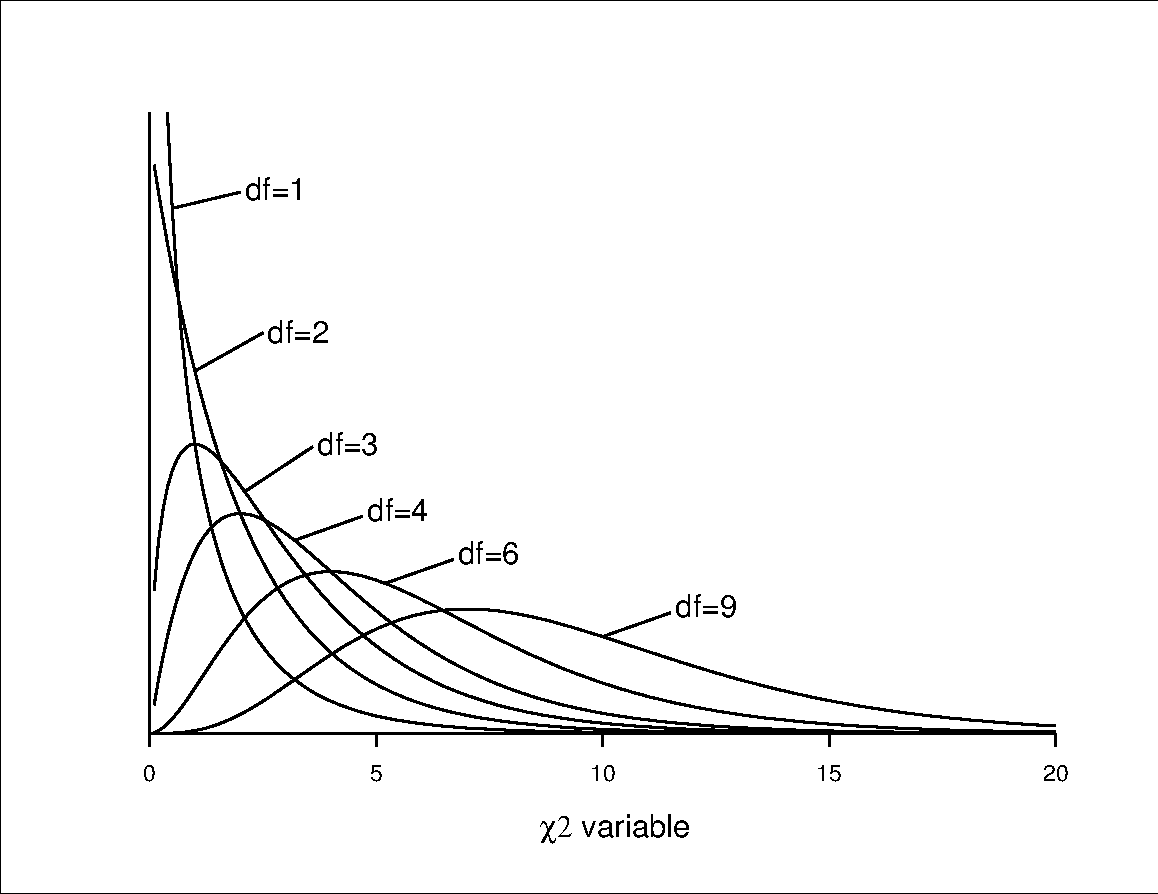
\includegraphics[width=115mm]{chi2dists}
\end{center}
\vspace*{-3ex}
\end{figure}

For the $\chi^{2}$  test statistic of
independence we have the following result:
\begin{itemize}
\item
When the null hypothesis (\ref{H0_chi2}) is true in the population, the
sampling distribution of the test statistic (\ref{chi2}) calculated for
a two-way table with $R$ rows and $C$ columns is approximately the $\chi^{2}$
distribution with $df=(R-1)(C-1)$ degrees of freedom.
\end{itemize}
The degrees of freedom are thus given by the number of rows in the table
minus one, multiplied by the number of columns minus one. Table
\ref{t_sex_attitude_ch4}, for example, has $R=2$ rows and $C=5$ columns,
so its degrees of freedom are $df=(2-1)\times(5-1)=4$ (as indicated by
the ``df'' column of the SPSS output of Figure \ref{f_spsschi2}). Figure
\ref{f_chisampld} shows the curve of the $\chi^{2}$ distribution with
$df=4$ superimposed on the histogram of the sampling distribution
obtained from the computer simulation. The two are in essentially
perfect agreement, as mathematical theory indicates they should be.

These degrees of freedom can be given a further interpretation which
relates to the structure of the table\footnote{In short, they are the
smallest number of cell frequencies such that they together with the row
and column marginal totals are enough to determine all the remaining
cell frequencies.}. We can, however, ignore this and treat $df$ simply
as a number which identifies the appropriate $\chi^{2}$ distribution to
be used for the $\chi^{2}$ test for a particular table. Often it is
convenient to use the notation $\chi^{2}_{df}$ to refer to a specific
distribution, e.g.\ $\chi^{2}_{4}$ for  the $\chi^{2}$ distribution with
4 degrees of freedom.

The $\chi^{2}$ sampling distribution is ``approximate'' in that it is
an \emph{asymptotic approximation} which is exactly correct only if the
sample size is infinite and approximately correct when it is
sufficiently large. This is the reason for the conditions for the sizes
of the expected frequencies that were discussed on page
\pageref{p_chi2_fesize}. When these conditions are satisfied, the
approximation is accurate enough for all practical purposes and we use
the appropriate $\chi^{2}$ distribution as the sampling distribution.

On page \pageref{p_2reqs}, under requirement 2 for a good test
statistic, we mentioned that its sampling distribution under the null
hypothesis should be ``known'' and ``of convenient form''. We now know
that for the $\chi^{2}$ test it is a $\chi^{2}$ distribution.
The ``convenient form''  means that the sampling distribution
should not depend on too many specific features of the data at hand. For
the $\chi^{2}$ test, the approximate sampling distribution depends
(through the degrees of freedom) only on the size of the table but not
on the sample size or the marginal distributions of the two variables.
This is convenient in the right way, because it means that we can
use the same $\chi^{2}$ distribution for any table with a given number
of rows and columns, as long as the sample size is large enough for the
conditions on page \pageref{p_chi2_fesize} to be satisfied.

\subsection{The $P$-value}
\label{ss_tables_chi2test_Pval}

The last key building block of significance testing operationalises the
comparison between the observed value of a test statistic and its
sampling distribution under the null hypothesis. In essence, it provides
a way to determine whether the test statistic in the sample should be
regarded as ``large'' or ``not large'', and with this the measure of
evidence against the null hypothesis that is the end product of the
test:
\begin{itemize}
\item
\label{p_pval_ref}
The $\mathbf{P}$\textbf{-value} is the
probability, if the null hypothesis was true in the population, of
obtaining a value of the test statistic which provides as strong or
stronger evidence against the null hypothesis, and in the direction of
the alternative hypothesis, as the the value of the test statistic in
the sample actually observed.
\end{itemize}
The relevance of the phrase ``in the direction of the alternative
hypothesis'' is not apparent for the $\chi^{2}$ test, so we can ignore
it for the moment. As argued above, for this test it is large values of
the test statistic which indicate evidence against the null hypothesis
of independence, so the values that correspond to ``as strong or
stronger evidence'' against it are the ones that are as
large or larger than the observed statistic. Their probability is
evaluated from the $\chi^{2}$ sampling distribution defined above.

Figure \ref{f_pvalchisq} illustrates this calculation. It shows the
curve of the $\chi^{2}_{4}$ distribution, which is the relevant sampling
distribution for the test for the $2\times 5$ table in our example.
Suppose first, hypothetically, that we had actually observed the sample
in the lower part of Table \ref{t_sex_attitude_H0pop}, for which the
value of the test statistic is $\chi^{2}=2.84$. The $P$-value of the
test for this sample would then be the probability of values of 2.84
or larger, evaluated from the $\chi^{2}_{4}$ distribution.

For a probability curve like the one in Figure \ref{f_pvalchisq}, areas
under the curve correspond to probabilities. For example, the area under
the whole curve from 0 to infinity is 1, because a variable which
follows the $\chi^{2}_{4}$ distribution is certain to have one of these values.
Similarly, the probability that we need for the $P$-value for
$\chi^{2}=2.84$ is the area under the curve to the right of the value
2.84, which is shown in grey in Figure \ref{f_pvalchisq}. This is
$P=0.585$.

The test statistic for the real sample in Table \ref{t_sex_attitude_ch4}
was $\chi^{2}=18.86$, so the $P$-value is the combined probability of
this and all larger values. This is also shown in Figure
\ref{f_pvalchisq}. However, this area is not really visible in the plot
because 18.86 is far into the tail of the distribution where the
probabilities are low. The $P$-value is then also low, specifically
$P=0.0008$.

\begin{figure}
\caption{Illustration of the $P$-value
for a $\chi^{2}$ test statistic with 4 degrees of freedom and with
values $\chi^{2}=2.84$  (area of the grey region under the curve) and
$\chi^{2}=18.86$.}
\label{f_pvalchisq}
\begin{center}
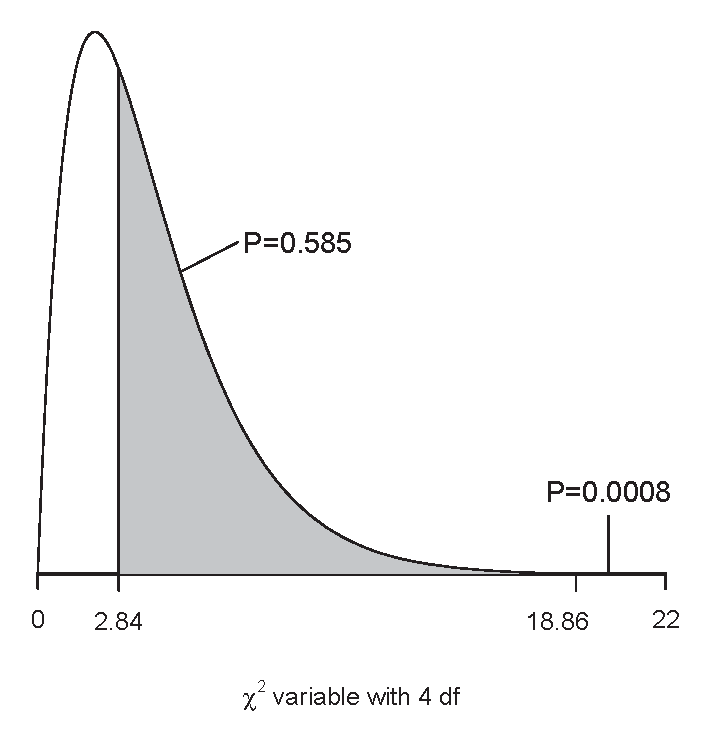
\includegraphics[width=8cm]{chi2_pval}
\end{center}
\vspace*{-3ex}
\end{figure}

\label{p_spss2b}
In practice the $P$-value is usually calculated by a computer. In the
SPSS output of Figure \ref{f_spsschi2} is is shown
in the column labelled ``Asymp.\ Sig. (2-sided)''
which is short for ``Asymptotic significance level'' (you can ignore the
``2-sided'' for this test). The value is listed as 0.001. SPSS reports,
by default, $P$-values rounded to three decimal places. Sometimes even
the smallest of these is zero, in which case the value is displayed
as ``.000''. This is bad practice, as the $P$-value for most
significance tests is never \emph{exactly} zero. $P$-values given by
SPSS as ``.000'' should be reported instead as ``$P<0.001$''.

Before the widespread availablity of statistical software, $P$-values
had to be obtained approximately using tables of distributions. Since
you may still see this approach described in many text books, it is
briefly explained here. You may also need to use the table method in the
examination, where computers are not allowed. Otherwise, however, this
approach is now of little interest: if the $P$-value is given in the
computer output, there is no need to refer to distributional tables.

All introductory statistical text books include a table of
$\chi^{2}$ distributions, although its format may vary
slightly form book to book. Such a table is also included on page
\pageref{s_disttables_chi2} of this coursepack. An extract from the
table is shown in Table \ref{t_chi2table}. Each row of the table
corresponds to a $\chi^{2}$ distribution with the degrees of freedom
given in the first column. The other columns show so-called ``critical
values'' for the probability levels given on the first row. Consider,
for example, the row for 4 degrees of freedom. The figure 7.78 in the
column for probability level 0.100 indicates that the probability of a
value of 7.78 or larger is exactly 0.100 for this distribution. The 9.49
in the next column shows that the probability of 9.49 or larger is
0.050. Another way of saying this is that if the appropriate degrees of
freedom were 4, and the test statistic was 7.78, the $P$-value would be
exactly 0.100, and if the statistic was 9.49, $P$ would be 0.050.

\begin{table}[t]
\caption{An extract from a table of critical values for
$\chi^{2}$ distributions.}
\label{t_chi2table}
\begin{center}
\begin{tabular}{|l|rrrr|}\hline
& \multicolumn{4}{|c|}{Right-hand tail probability} \\
df & 0.100 & 0.050 & 0.010 & 0.001 \\ \hline
1 & 2.71 & 3.84 & 6.63 & 10.83 \\
2 & 4.61 & 5.99 & 9.21 & 13.82 \\
3 & 6.25 & 7.81 & 11.34 & 16.27 \\
4 & 7.78 & 9.49 & 13.28 & 18.47 \\
$\vdots$ & $\vdots$ & &  & $\vdots$ \\
\hline
\end{tabular}
\end{center}
\end{table}

The values in the table also provide bounds for other
values that are not shown. For instance, in the hypothetical sample in
Table \ref{t_sex_attitude_H0pop} we had $\chi^{2}=2.84$, which is
smaller than 7.78. This implies that the corresponding $P$-value must be
larger than 0.100, which (of course) agrees with the precise value of
$P=0.585$ (see also Figure \ref{f_pvalchisq}). Similarly,
$\chi^{2}=18.86$ for the real
data in Table \ref{t_sex_attitude_ch4}, which
is larger than the 18.47 in the ``0.001'' column of the table for the
$\chi^{2}_{4}$ distribution. Thus the corresponding $P$-value must be
smaller than 0.001, again agreeing with the correct value of $P=0.0008$.

\subsection{Drawing conclusions from a test}
\label{ss_tables_chi2test_conclusions}

The $P$-value is the end product of any significance test, in that it is
a complete quantitative summary of the strength of evidence against the
null hypothesis provided by the data in the sample. More precisely, the
$P$-value indicates how likely we would be to obtain a value of the test
statistic which was as or more extreme as the value for the data, if the
null hypothesis was true. Thus the \emph{smaller} the $P$-value, the
stronger is the evidence \emph{against} the null hypothesis. For
example, in our survey example of sex and attitude toward income
redistribution we obtained $P=0.0008$ for the $\chi^{2}$ test of
independence. This is a small number, so it indicates strong evidence
against the claim that the distributions of attitudes are the same for
men and women in the population.

For many purposes it is quite sufficient to simply report the $P$-value.
It is, however, quite common also to state the conclusion in the form of
a more discrete decision of ``rejecting'' or ``not rejecting'' the null
hypothesis. This is usually based on conventional reference levels,
known as \textbf{significance levels} or
$\boldsymbol{\alpha}$\textbf{-levels}
(here $\alpha$ is the lower-case
Greek letter ``alpha''). The standard significance levels are 0.10,
0.05, 0.01 and 0.001 (also known as 10\%, 5\%, 1\% and 0.1\%
significance levels respectively), of which the 0.05 level is most
commonly used; other values than these are rarely considered. The values of the
test statistic which correspond exactly to these levels are the critical
shown in the table of the $\chi^{2}$ distribution in Table
\ref{t_chi2table}.

When the $P$-value is \emph{smaller} than a conventional level of
significance (i.e.\ the test statistic is \emph{larger} than the
corresponding critical value), it is said that the null hypothesis is
\textbf{rejected} at that level of significance, or that the results
(i.e.\ evidence against the null hypothesis) are \textbf{statistically
significant} at that level. In our example the $P$-value was smaller
than 0.001. The null hypothesis is thus ``rejected at the 0.1 \% level of
significance'', i.e.\ the evidence that the variables are not
independent in the population is ``statistically significant at the
0.1\% level'' (as well as the 10\%, 5\% and 1\% levels of course, but it
is enough to state only the strongest level).

The strict decision formulation of significance testing is much overused
and misused. It is in fact quite rare that the statistical analysis will
immediately be followed by some practical action which absolutely
requires a decision about whether to act on the basis of the null
hypothesis or the alternative hypothesis. Typically the analysis which a
test is part of aims to examine some research question, and the results
of the test simply contribute new information to add support for one or
the other side of the argument about the question. The $P$-value is the
key measure of the strength and direction of that evidence, so it should
\emph{always} be reported. The standard significance levels used for
rejecting or not rejecting null hypotheses, on the other hand, are
merely useful conventional reference points for structuring the
reporting of test results, and their importance should not be
overemphasised. Clearly $P$-values of, say, 0.049 and 0.051 (i.e.\ ones
either side of the most common conventional significance level 0.05)
indicate very similar levels of evidence against a null hypothesis, and
acting as if one was somehow qualitatively more decisive is simply
misleading.

\subsubsection{How to state the conclusions}

The final step of a significance test is describing its conclusions in a
research report. This should be done with appropriate care:
\begin{itemize}
\item
The report should make clear which test was used. For example, this
might be stated as something like ``The $\chi^{2}$ test of independence
was used to test the null hypothesis that in the population the attitude toward income
redistribution was independent of sex in the population''.
There is usually no need to give literature references
for the standard tests described on this course.
\item
The numerical value of the $P$-value should be reported, rounded
to two or three decimal places (e.g.\ $P=0.108$ or $P=0.11$). It can
also reported in an approximate way
as, for example, ``$P<0.05$'' (or the
same in symbols to save space,
e.g.\ * for $P<0.1$, ** for $P<0.05$, and so on). Very small
$P$-values can always be reported as
something like ``$P<0.001$''.
\item
When (cautiously) discussing the results in terms of discrete decisions,
the most common practice is to say that the null hypothesis was either
\emph{not rejected} or \emph{rejected} at a given significance level. It
is \emph{not} acceptable to say that the null hypothesis was
``accepted'' as an alternative to ``not rejected''. Failing to reject
the hypothesis that two variables are independent in the population
is not the same as proving that they actually \emph{are} independent.
\item
A common mistake is to describe the $P$-value as the probability that
the null hypothesis is true. This is understandably tempting, as such a
claim would seem more natural and convenient than the correct but convoluted
interpretation of the $P$-value as ``the probability of obtaining a test
statistic as or more extreme as the one observed in the data if the test
was repeated many times for different samples from a population where
the null hypothesis was true''. Unfortunately, however, the $P$-value is
\emph{not} the probability of the null hypothesis being true. Such a
probability does not in fact have any real meaning at all in the
statistical framework considered here\footnote{There is an alternative
framework, known as \emph{Bayesian} statistics,
where quantities resembling $P$-values \emph{can} be
given this interpretation. The differences between the Bayesian
approach and the so-called \emph{frequentist} one discussed here are
practically and philosophically important and interesting, but beyond the scope of
this course.}.
\item
The results of significance tests should be stated
using the names and values of the variables involved, and
not just in terms of
``null'' and ``alternative'' hypotheses. This also forces you
to recall what the hypotheses actually were, so that you do not
accidentally describe the
result the wrong way round (e.g.\ that the data support a claim when
they do just the opposite). There are no
compulsory phrases for stating the conclusions, so it can be done in a
number of ways. For example, a fairly complete and careful statement
in our example would be
\begin{itemize}
\item
``There is strong
evidence that the distributions of attitudes toward income
redistribution are not the same
for men and women in the population
($P<0.001$).''
\end{itemize}
Other possibilities are
\begin{itemize}
\item
``The association between sex and attitude toward income redistribution
in the sample is statistically
significant ($P<0.001$).''
\item
``The analysis suggests that there is an association
between sex and attitude toward income redistribution
in the population
($P<0.001$).''
\end{itemize}
The last version is slightly less clear than the other statements in that it relies
on the reader recognizing that the inclusion of the $P$-value implies
that the word ``differs'' refers to a statistical claim rather a
statement of absolute fact about the population. In many contexts it
would be better to say this more explicitly.
\end{itemize}
Finally, if the null hypothesis of independence is rejected, the test
should not usually be the only statistical analysis that is reported
for a two-way table. Instead, we would then go on to describe
\emph{how} the two variables appear to be associated, using the of
descriptive methods discussed in Section
\ref{s_descr1_2cat}.

\section{Summary of the $\chi^{2}$ test of independence}
\label{s_tables_summary}

We have now described the elements of a significance test in some
detail. Since it is easy to lose sight of the practical steps of a test
in such a lengthy discussion, they are briefly repeated here for the
$\chi^{2}$ test of independence.
The test of
the association between sex and attitude in the survey example is again used for illustration:
\begin{enumerate}
\item
Data: observations of two categorical variables, here sex and
attitude towards income redistribution for $n=2344$ respondents, presented in
the two-way, $2\times 5$ contingency table \ref{t_sex_attitude_ch4}.
\item
Assumptions: the variables can have any measurement level, but the expected
frequencies $f_{e}$ must be large enough. A common rule of thumb is that
$f_{e}$ should be at least 5 for every cell of the table. Here the
smallest expected frequency is 32.9, so the requirement is comfortably
satisfied.
\item
Hypotheses: null hypothesis $H_{0}$ that the two
variables are statistically independent (i.e.\ not associated) in the
population, against the alternative hypothesis that they are dependent.
\item
The test statistic: the $\chi^{2}$ statistic
\[
\chi^{2} = \sum
\frac{(f_{o}-f_{e})^{2}}{f_{e}}
\]
where $f_{o}$ denotes observed
frequencies in the cells of the table and $f_{e}$ the corresponding
expected frequencies under the null hypothesis,
and the summation is over all of the cells. For Table
\ref{t_sex_attitude_ch4}, $\chi^{2}=18.86$.
\item
The sampling distribution of
the test statistic when $H_{0}$ is true: a $\chi^{2}$ distribution with
$(R-1)\times(C-1)=1\times 4=4$ degrees of freedom, where $R$ $(=2)$ and
$C$ $(=5)$ denote the numbers of rows and columns in the table
respectively.
\item
The $P$-value: the probability that a randomly
selected value from the $\chi^{2}_{4}$ distribution is at least 18.86.
This is $P=0.0008$, which may also be reported as $P<0.001$.
\item
Conclusion: the null hypothesis of independence is strongly rejected.
The $\chi^{2}$ test indicates very strong evidence that sex and
attitude towards income redistribution are associated in the population
($P<0.001$).
\end{enumerate}
When the association is judged to be
statistically significant, its nature and magnitude can be further
explored using the descriptive methods for two way tables discussed in Section
\ref{s_descr1_2cat}.


